\chapter{Endgame Solving}
\label{ch:endgame-solving}
\epigraph{
  Poker has the only river in the world you can drown in more than once.
}{an~old Poker joke}
\vskip -2em
\note{
  This chapter summarizes the approach, methods and results of~the authors \cite{Ganzfried2015endgame}.
}

\section{Motivation}
\epigraphLong{
  Memorizing a~playbook is like memorizing a~script.
  When they change the script at the last minute it's like changing a~play in~a~game.
}{Michael Strahan}
Two-player zero-sum imperfect-information games can be solved via linear programming (\cite{Koller1994fast}), by modelling sequences of~moves as variables of~a~sequence-form \acrshort{lp} (recall Section~\ref{sec:solving-games-lp}).
This approach scales well to games with up to $10^8$ game states.
Unfortunately, many attractive Poker games are far larger~(\cite{Johanson2013measuring}):
\begin{itemize}
  \item two-player \acrfull{lhe} $\approx 10^{17}$ states
  \item two-player \acrfull{nlhe}\footnotemark{} $\approx 10^{165}$ states.
    \footnotetext{the most popular online variant of~Poker}
\end{itemize}
It is possible to find approximate equilibrium with iterative algorithms, as well.
These methods are guaranteed to converge in~the limit, and scale to~at least $10^{12}$ states (\cite{Hoda2010smoothing}; \cite{Zinkevich2007regret}).
Nevertheless, that is still not enough for the mentioned big poker variants.

Today, a~prevailing approach to enormous imperfect-information games (such as \acrshort{lhe} or \acrshort{nlhe}) is to reduce their sizes by~means of~\emph{abstractions}:
\begin{description}
  \item [Information abstraction] groups together different signals (e.g. similar poker hands).
  \item [Action abstraction] discretizes an~immense action space, making it thus smaller and more manageable.
\end{description}
The method afterwards finds an~\emph{approximate equilibrium} in the abstracted game.

An~appealing idea to diminish harmful effects of~the abstraction and the approximate-equilibrium search, is to~solve endgames dynamically:
an~agent only needs to~deal with those portions of~the game that are actually reached during a~play.
As a~consequence, the endgame can be re-solved with a~finer abstraction and more precise pot and stack sizes.

\section{Gadget Game}
\epigraphLong{
  What is so brilliant about the gadgets is their simplicity.
}{Desmond Llewelyn}
We start by~constructing a~fine-grained subgame abstraction.
The original strategies for the subgame are discarded and only the strategies prior to the subgame (i.e. the trunk) are needed.
The strategies in the trunk are used to compute the joint distribution (i.e. belief) over the states at~the beginning of the subgame.

Finally, we add a~chance node~$c$ just before the fine-grained subgame~$S$.
The node leads to the states at~the root of~the subgame.
The chance node plays according to the computed belief.
Adding the chance node ``roots'' the subgame, thus making it a~proper tree of a~well-defined game (Figure~\ref{fig:endgame-solving-gadget}).
\begin{figure}[H]
  \centering
  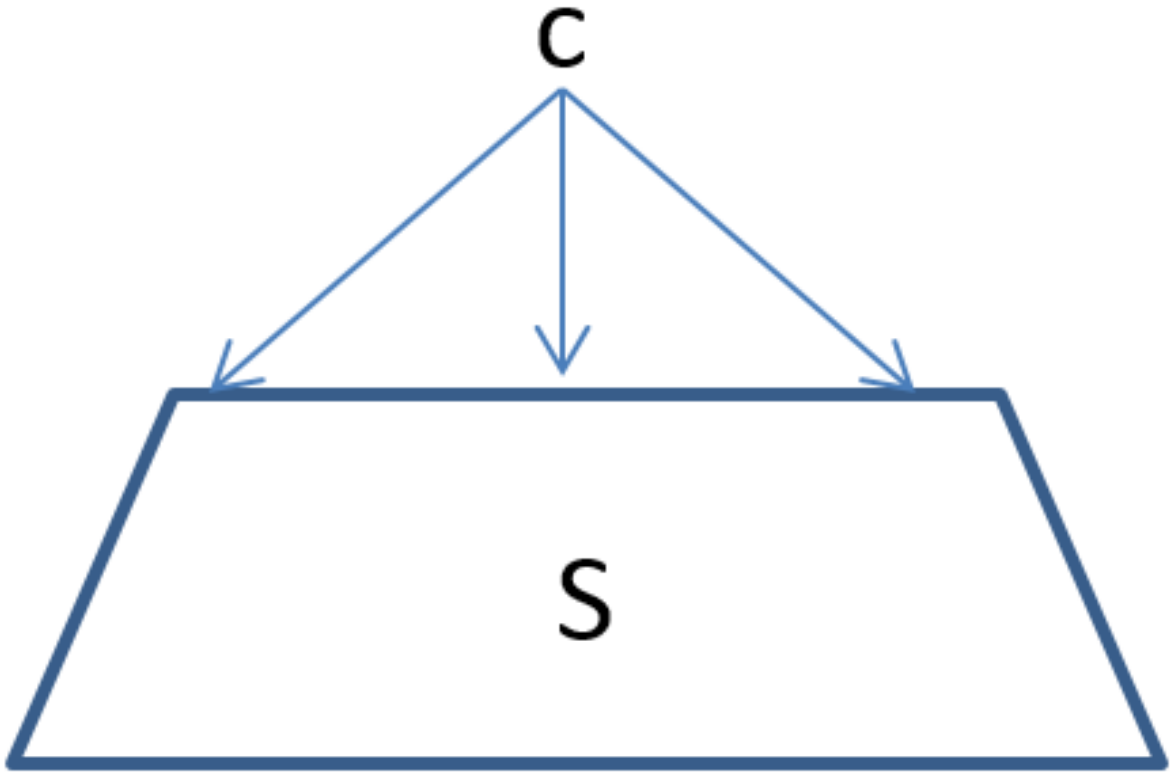
\includegraphics[width=.3\textwidth]{../img/endgame-solving-gadget.png}
  \caption{A~gadget game for endgame solving}
  \label{fig:endgame-solving-gadget}
\end{figure}

\section{Equivalent Linear Program}
The equivalent \acrshort{lp} formulation for the abstracted endgame is the sequence-form \acrshort{lp} from~(\ref{lp:seq-form}):
\begin{equation*}
  \label{lp:endgame-solving}
  \begin{split}
    \max_{v, x}\  f^\top v & \\
    Ex &= e \\
    F^\top v - A_{\color{red}2}^\top x &\le \vect{0} \\
    x &\ge \vect{0},
  \end{split}
\end{equation*}

\todo

\section{Discussion}
The endgame solving improves agents' play only \emph{empirically}~(\cite[Table~1]{Ganzfried2015endgame}).
Theoretically, however, there is no guarantee of~optimality:
even if the trunk strategy (and thus the starting distribution) is optimal, the combined strategy can become drastically more exploitable.
This undesired effect is noticeable in~the extensive form of~rock-paper-scissors (Claim~\ref{claim:rps-subgame}, Chapter~\ref{ch:imperf-shortcomings}).

A~worse exploitability arises when the opponent can ``see a~better option'' and aim for it.
This notion of~a~better alternative can be summarized by~a~\emph{counterfactual value}, and Chapter~\ref{ch:cfr-d} shows how to use these values to~guarantee theoretical bounds.
